\documentclass[conference]{IEEEtran}
\IEEEoverridecommandlockouts
% The preceding line is only needed to identify funding in the first footnote. If that is unneeded, please comment it out.
% Template version as of 6/27/2024

% --- Paquetes para soporte de idioma espanol (acentos y "n") ---
\usepackage[utf8]{inputenc}
\usepackage[T1]{fontenc}
% ---------------------------------------------------------------

\usepackage{cite}
\usepackage{amsmath,amssymb,amsfonts}
\usepackage{algorithmic}
\usepackage{graphicx}
\usepackage{textcomp}
\usepackage{xcolor}
\usepackage{booktabs}
\def\BibTeX{{\rm B\kern-.05em{\sc i\kern-.025em b}\kern-.08em
    T\kern-.1667em\lower.7ex\hbox{E}\kern-.125emX}}
\begin{document}

\title{Personalizacion de Menus en Sistemas ERP mediante Modelos Neuronales Secuenciales y Agentes DQN: un Enfoque Auto-Adaptativo\\
{\footnotesize Un estudio empirico sobre la reduccion del costo de navegacion en interfaces empresariales}
}

\author{\IEEEauthorblockN{1\textsuperscript{st} Jose Samuel Turpo Cauna}
\IEEEauthorblockA{\textit{Facultad de Ingenieria y Arquitectura} \\
\textit{Universidad Peruana Union (UPeU)}\\
Juliaca, Peru \\
jose.turpo.c@upeu.edu.pe}
\and
\IEEEauthorblockN{2\textsuperscript{nd} Jhosef Anthony Quispe Huarilloclla}
\IEEEauthorblockA{\textit{Facultad de Ingenieria y Arquitectura} \\
\textit{Universidad Peruana Union (UPeU)}\\
Juliaca, Peru \\
jhosef.quispe@upeu.edu.pe}
\and
\IEEEauthorblockN{3\textsuperscript{rd} Yesenia Alejandra Gutierrez Anco}
\IEEEauthorblockA{\textit{Facultad de Ingenieria y Arquitectura} \\
\textit{Universidad Peruana Union (UPeU)}\\
Juliaca, Peru \\
yesenia.gutierrez@upeu.edu.pe}
}

\maketitle

\begin{abstract}
Los sistemas ERP concentran gran parte de sus funciones en menus jerarquicos profundos, lo que incrementa el costo de navegacion del usuario y su carga cognitiva. Este trabajo presenta un enfoque auto-adaptativo que personaliza los menus de un ERP de gestion de articulos combinando un modelo neuronal secuencial de prediccion de la siguiente ruta con un agente de aprendizaje por refuerzo profundo del tipo Deep Q-Network (DQN) que reestructura el orden de los items. A partir de un corpus real de 87465 eventos de interaccion agrupados en 1206 sesiones de ocho usuarios y cuatro roles, se compararon cuatro arquitecturas predictivas (LSTM, GRU, Transformer y CNN 1D). La red GRU obtuvo la mejor exactitud sobre el vocabulario completo de 44 rutas (Top-1 de 0.3838 y Top-3 de 0.7294) con la convergencia mas rapida, por lo que fue seleccionada como generadora del puntaje de relevancia que alimenta al agente DQN. La probabilidad predictiva de la GRU se integro con la senal de recompensa del DQN mediante un puntaje compuesto ponderado. En una validacion PRE/POST, el numero de clics (M1) se redujo un 19.09\% (p menor que 0.001; d de Cohen igual a 0.646) y la tasa de error (M3) un 28.94\% (p menor que 0.001; d igual a 0.713), ambos con efecto medio y estadisticamente significativos; el tiempo de tarea (M2) disminuyo un 28.95\% pero sin significancia estadistica (p igual a 1.0; d igual a 0.284). Los resultados sugieren que la integracion de prediccion secuencial y reestructuracion por refuerzo reduce de forma medible el esfuerzo de navegacion, aunque no alcanza la meta autoimpuesta del 30\% de reduccion de clics.
\end{abstract}

\begin{IEEEkeywords}
sistemas auto-adaptativos, aprendizaje por refuerzo, Deep Q-Network, interfaces adaptativas, personalizacion de menus, sistemas ERP, redes neuronales recurrentes, GRU
\end{IEEEkeywords}

\section{Introduccion}
Los sistemas de planificacion de recursos empresariales (ERP) integran procesos de ventas, compras, caja, logistica y reportes en una unica plataforma. Esta amplitud funcional se traduce en menus jerarquicos extensos y profundos que el usuario debe recorrer repetidamente, incrementando el numero de clics, el tiempo de tarea y la probabilidad de error. La optimizacion de la disposicion de estos menus es un problema clasico de interaccion humano-computadora, donde una adaptacion mal escogida puede imponer costos elevados al usuario debido a la sorpresa o al esfuerzo de reaprendizaje \cite{b_todi}. En la practica, el ERP tratado en este estudio organiza sus opciones en un vocabulario de 44 rutas de navegacion distribuidas en cuatro roles operativos.

Las interfaces de usuario adaptativas (AUI) han sido abordadas desde la ingenieria de sistemas auto-adaptativos (SAS), donde un lazo de retroalimentacion permite que el sistema afronte la incertidumbre de operacion, tal como propone el paradigma MAPE-K y sus realizaciones formales en tiempo de ejecucion \cite{b_activforms,b_kephart}. En paralelo, el aprendizaje por refuerzo (RL) se ha consolidado como una tecnica efectiva para personalizar interfaces, ya que optimiza una politica a partir de la interaccion continua con el entorno \cite{b_sunxue,b_troussas}. Sin embargo, gran parte de los trabajos previos evaluan interfaces genericas o de escritorio y rara vez abordan menus ERP con restricciones por rol, ni cuantifican el impacto con un diseno estadistico PRE/POST.

Este articulo propone y evalua un enfoque hibrido de dos etapas. Primero, un modelo neuronal secuencial predice la siguiente ruta que el usuario visitara a partir de su historial de interaccion, produciendo un puntaje de relevancia por item. Segundo, un agente DQN reestructura el orden de los items del menu, tratando la reordenacion como un problema de decision secuencial cuyo objetivo es minimizar el costo de navegacion. La contribucion principal es empirica: (i) una comparacion objetiva de cuatro arquitecturas predictivas sobre un corpus real de un ERP en produccion; (ii) la integracion del predictor secuencial con un agente DQN mediante un puntaje compuesto; y (iii) una validacion estadistica del impacto sobre tres metricas de costo de navegacion (clics, tiempo y error).

\section{Trabajos Relacionados}
La adaptacion de interfaces mediante aprendizaje por refuerzo ha sido explorada de forma prominente por Todi \textit{et al.}, quienes plantean menus adaptativos basados en un RL con modelo que planifica secuencias de adaptaciones y consulta modelos predictivos de HCI para estimar sus efectos, superando politicas no adaptativas y de frecuencia \cite{b_todi}. Sun y Xue proponen una generacion adaptativa de interfaces guiada por RL con realimentacion inteligente, evaluada mediante tasa de clics y retencion \cite{b_sunxue}, mientras que Troussas \textit{et al.} combinan logica difusa y RL para ajustar dinamicamente los pesos de una interfaz educativa \cite{b_troussas}. Estos trabajos confirman la pertinencia del RL para la personalizacion, pero se centran en dominios distintos al ERP.

Desde la perspectiva de los SAS, ActivFORMS aporta un enfoque de extremo a extremo con modelos formales activos y verificacion en tiempo de ejecucion para garantizar los objetivos de adaptacion \cite{b_activforms}, y Wohlrab \textit{et al.} abordan la adaptacion en tiempo de ejecucion de atributos de calidad para la planificacion automatizada \cite{b_wohlrab}. La adaptacion sensible al contexto para incrementar la conciencia situacional, combinando modelado ontologico y optimizacion combinatoria, fue propuesta por Stefanidi \textit{et al.} \cite{b_stefanidi}. Una revision sistematica reciente sobre aprendizaje automatico para interfaces accesibles adaptativas evidencia el predominio del aprendizaje supervisado y las oportunidades del RL \cite{b_kristic}, y estudios de experiencia de usuario comparan desempeno y preferencias en interfaces adaptativas \cite{b_gaspar}. En el ambito especifico de menus, Sahraoui \textit{et al.} introducen los menus adaptativos fractales que explotan la auto-similitud y la navegacion recursiva \cite{b_fractal}.

El modelado de la navegacion del usuario como proceso secuencial tiene una base solida en la mineria de secuencias. Aung y Kumoi modelan las trayectorias de usuarios web con cadenas de Markov absorbentes de primer orden para optimizar la conversion \cite{b_aung}; Chen \textit{et al.} aplican modelado de Markov embebido para minar rutas de navegacion en guias electronicas \cite{b_chen}; y Alamoudi \textit{et al.} predicen patrones de clickstream en entornos ruidosos mediante modelos ocultos de Markov \cite{b_alamoudi}. En el contexto ERP, Suleiman y Kassem emplean mineria de procesos y RPA cognitiva para automatizar tareas de entrada de datos \cite{b_suleiman}, y la optimizacion de la carga cognitiva en el diseno de interfaces ha sido estudiada para servicios de informacion \cite{b_balasm}. Este trabajo se apoya en esa tradicion secuencial, pero reemplaza los modelos de Markov por redes neuronales que capturan dependencias de mayor orden, y acopla la prediccion con un agente DQN de reestructuracion. Los autores han explorado previamente la adaptacion dinamica de interfaces empresariales con GRU y DQN bajo restricciones RBAC \cite{b_prev}.

\section{Materiales y Metodos}

\subsection{Corpus y metricas base (OE1)}
El corpus se construyo a partir de los registros de interaccion del ERP durante el periodo comprendido entre enero y abril de 2026. Contiene 87465 eventos agrupados en 1206 sesiones, generados por ocho usuarios distribuidos en cuatro roles (Administrador, Ventas, Compras y Almacen), sobre un vocabulario de 44 rutas de navegacion. Se definieron tres metricas de costo de navegacion: el numero promedio de clics hasta alcanzar el destino (M1), el tiempo de tarea en segundos (M2) y la tasa de error de navegacion (M3). La linea base sobre el corpus completo fue M1 igual a 2.978 clics, M2 igual a 302.286 s y M3 igual a 0.2888, con perfiles de frecuencia normalizada por usuario y rol que sirvieron como estado inicial del sistema.

\subsection{Modelos neuronales secuenciales (OE2)}
El problema de prediccion se formulo como la estimacion de la siguiente ruta $r_{t+1}$ dado el historial de las ultimas rutas visitadas. Se fijo una longitud de secuencia de 10 pasos y una capa de \textit{embedding} de dimension 32. Se entrenaron y compararon cuatro arquitecturas: LSTM, GRU, Transformer y CNN 1D. Todas comparten el mismo vocabulario de 44 clases y fueron evaluadas con perdida de entropia cruzada y exactitud de validacion. Adicionalmente, para las dos arquitecturas finalistas se computo la exactitud Top-1 y Top-3 sobre el conjunto de prueba con el vocabulario completo, metrica que constituye el criterio de seleccion definitivo por reflejar la utilidad real de la recomendacion.

La probabilidad predictiva del modelo ganador se convierte en un puntaje de relevancia $s_i$ por item. Este puntaje se integra despues con la senal del agente de refuerzo mediante una combinacion lineal ponderada
\begin{equation}
s_i = \alpha\, p^{\text{seq}}_i + \beta\, f_i + \gamma\, q_i,\label{eq_score}
\end{equation}
donde $p^{\text{seq}}_i$ es la probabilidad entregada por el modelo secuencial, $f_i$ la frecuencia historica normalizada y $q_i$ el valor aprendido por el agente; los pesos empleados fueron $\alpha = 0.5$, $\beta = 0.3$ y $\gamma = 0.2$.

\subsection{Agente DQN de reestructuracion (OE3)}
La reordenacion del menu se modelo como un proceso de decision de Markov y se resolvio con un agente Deep Q-Network (DQN) \cite{b_mnih}, entrenado con una recompensa moldeada (\textit{shaped reward}) que premia colocar las rutas de mayor relevancia en las primeras posiciones y penaliza el costo de navegacion resultante. Se entrenaron agentes independientes segun el tamano del grupo de items a ordenar (1, 2, 4, 6 y 9 items) para estudiar el efecto de la dimension del espacio de acciones sobre la convergencia. El resultado de esta etapa es un conjunto de menus personalizados por rol y usuario.

\subsection{Implementacion, robustez y validacion (OE4 y OE5)}
La implementacion se sometio a un conjunto de pruebas de entorno, robustez y privacidad. El impacto final se evaluo con un diseno PRE/POST sobre las tres metricas de costo de navegacion, reportando las medias antes y despues, la significancia estadistica y el tamano del efecto mediante la $d$ de Cohen \cite{b_cohen}. El fundamento teorico del aprendizaje por refuerzo sigue la formulacion estandar de Sutton y Barto \cite{b_sutton}; las arquitecturas recurrentes con compuertas y la atencion siguen, respectivamente, a Cho \textit{et al.} \cite{b_cho} y Vaswani \textit{et al.} \cite{b_vaswani}.

\section{Resultados}

\subsection{Seleccion del modelo secuencial}
La Tabla~\ref{tab_modelos} sintetiza la comparacion de las cuatro arquitecturas. En terminos de la exactitud de validacion utilizada como aproximacion durante el entrenamiento, los cuatro modelos alcanzan valores cercanos (entre 0.496 y 0.502), lo que indica que la senal de la siguiente ruta es intrinsecamente dificil de predecir de forma exacta en un vocabulario de 44 clases. El criterio decisivo fue la exactitud Top-1 y Top-3 sobre el vocabulario completo, disponible para las dos arquitecturas finalistas: la red GRU supera al Transformer tanto en Top-1 (0.3838 frente a 0.3543) como en Top-3 (0.7294 frente a 0.7101). Ademas, la GRU alcanzo su mejor exactitud de validacion en la epoca 15, frente a las epocas 34 a 37 de las demas arquitecturas, evidenciando una convergencia sensiblemente mas rapida.

\begin{table}[htbp]
\caption{Comparacion de arquitecturas secuenciales (OE2)}
\begin{center}
\begin{tabular}{lccccc}
\toprule
\textbf{Modelo} & \textbf{Val.\ acc.} & \textbf{Val.\ loss} & \textbf{Ep.\ conv.} & \textbf{Top-1} & \textbf{Top-3} \\
\midrule
LSTM        & 0.5015 & 1.1351 & 37 & --     & --     \\
CNN 1D      & 0.4988 & 1.1386 & 34 & --     & --     \\
Transformer & 0.4961 & 1.1451 & 36 & 0.3543 & 0.7101 \\
\textbf{GRU}$^{\mathrm{a}}$ & 0.4989 & 1.1415 & \textbf{15} & \textbf{0.3838} & \textbf{0.7294} \\
\bottomrule
\multicolumn{6}{l}{\footnotesize $^{\mathrm{a}}$Modelo seleccionado. Val.\ acc.: mejor exactitud de validacion;}\\
\multicolumn{6}{l}{\footnotesize Ep.\ conv.: epoca de la mejor exactitud; Top-k sobre 44 rutas.}\\
\end{tabular}
\label{tab_modelos}
\end{center}
\end{table}

Por la combinacion de mayor exactitud Top-1/Top-3 sobre el vocabulario completo, convergencia mas rapida y un tamano compacto (\textit{embedding} de 32 y estado oculto de 64 unidades), la GRU se selecciono como generadora del puntaje de relevancia integrado con el agente DQN. Esta eleccion favorece la inferencia en tiempo real requerida para adaptar el menu en cada solicitud. La Fig.~\ref{fig_oe2} muestra las curvas de perdida y de exactitud Top-1 de las dos finalistas, donde la ventaja consistente de la GRU en validacion es visible a lo largo de todo el entrenamiento.

\begin{figure}[htbp]
\centerline{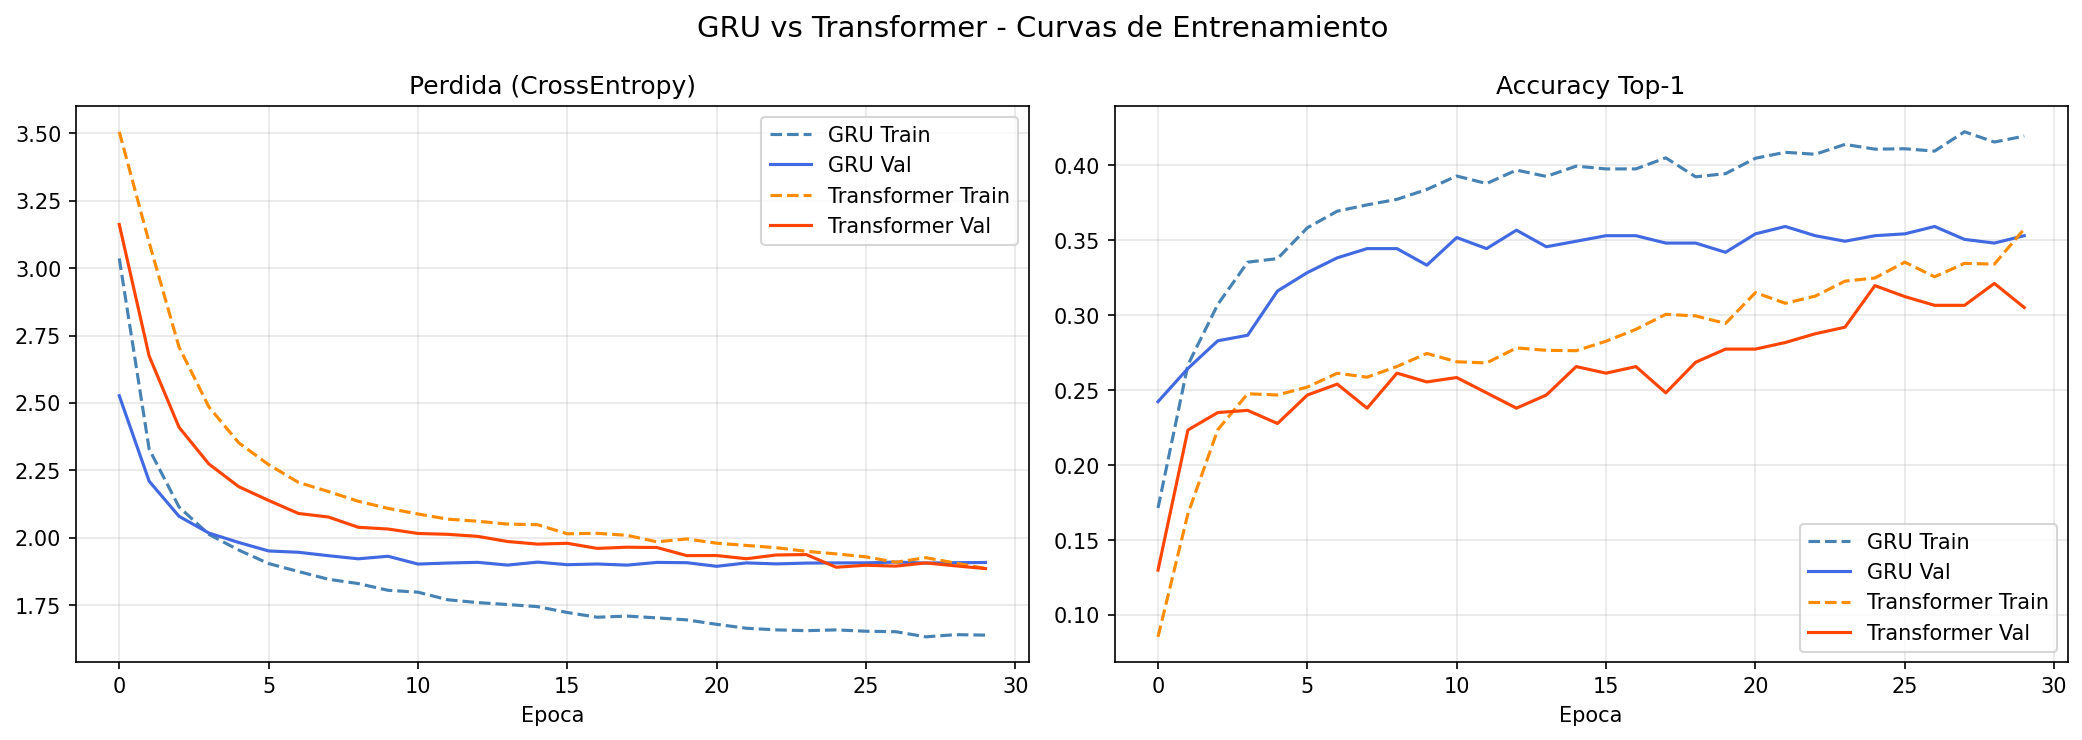
\includegraphics[width=\columnwidth]{fig_oe2_modelos.png}}
\caption{Curvas de entrenamiento de las arquitecturas finalistas (OE2). Izquierda: perdida de entropia cruzada. Derecha: exactitud Top-1. La GRU (azul) domina al Transformer (rojo) en validacion.}
\label{fig_oe2}
\end{figure}

\subsection{Entrenamiento del agente DQN y reestructuracion}
Se generaron 28 menus personalizados. La Fig.~\ref{fig_oe3} presenta la recompensa moldeada por episodio para cada tamano de grupo. Los grupos de 1, 2 y 4 items convergen al valor optimo, el grupo de 6 items se estabiliza cerca del optimo con oscilaciones ocasionales, y el grupo de 9 items alcanza una recompensa notablemente menor, lo que refleja el crecimiento combinatorio del espacio de acciones y la mayor dificultad de ordenar grupos grandes.

\begin{figure}[htbp]
\centerline{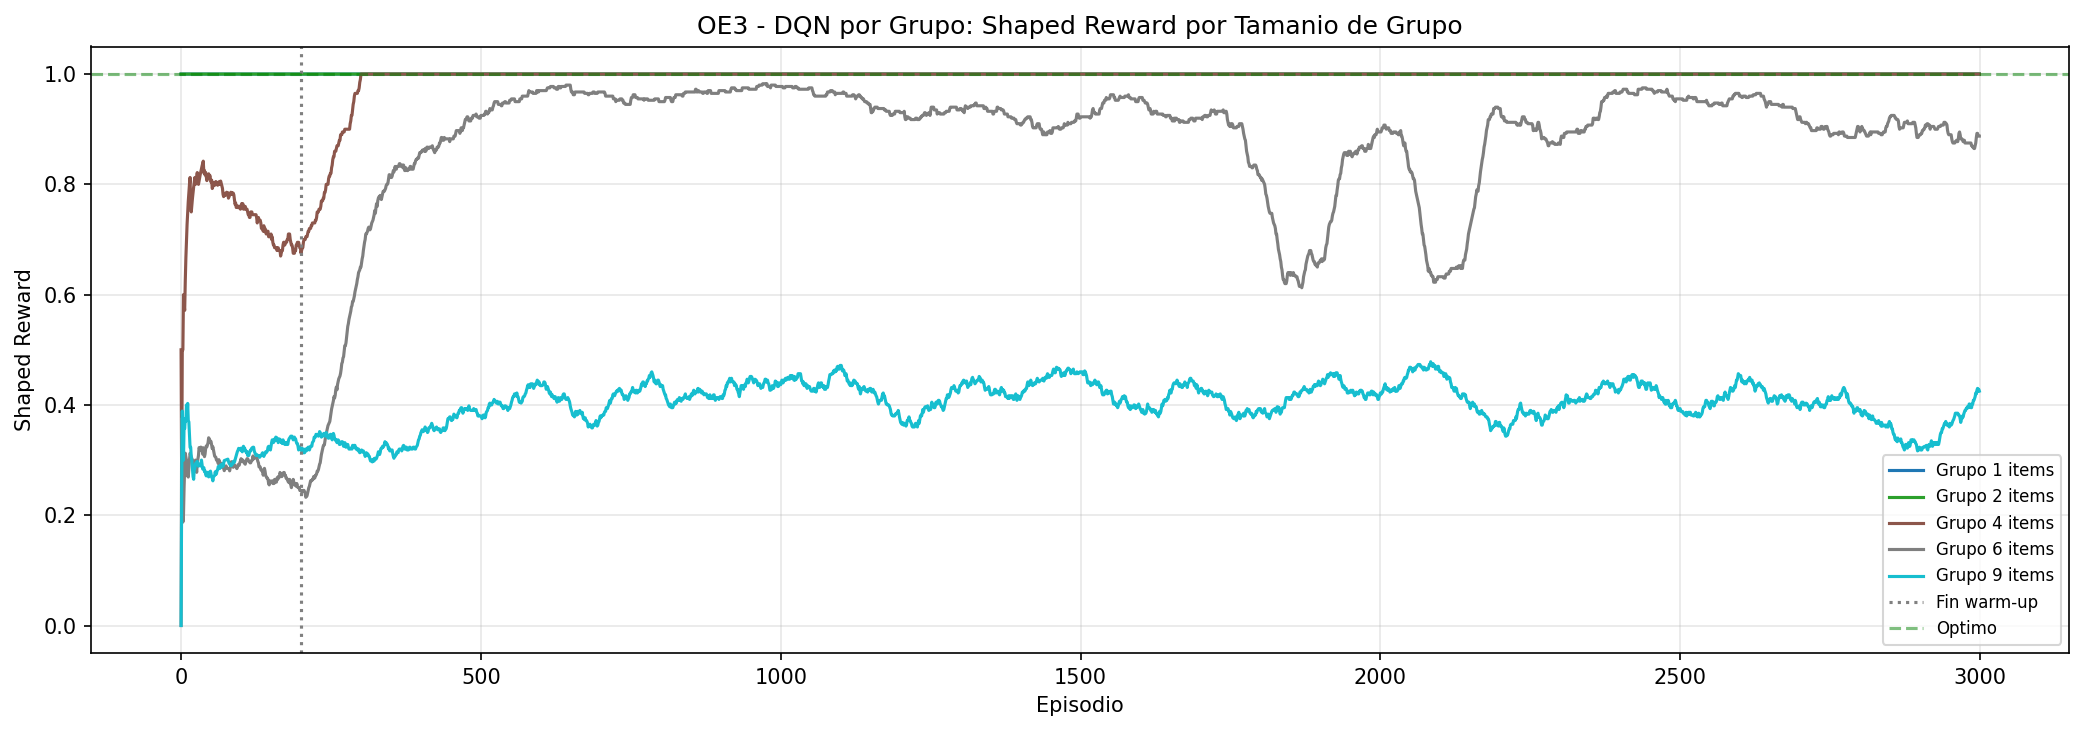
\includegraphics[width=\columnwidth]{fig_oe3_dqn.png}}
\caption{Recompensa moldeada del agente DQN por episodio, segun el tamano del grupo de items a reordenar (OE3). La dificultad de convergencia crece con el numero de items.}
\label{fig_oe3}
\end{figure}

Sobre el conjunto de 28 menus, la reduccion promedio del numero de clics (M1) fue de 22.26\%, con un maximo de 47.74\% y un minimo de 7.00\%. El desglose por rol revela una heterogeneidad marcada: el rol de Caja obtuvo la mayor reduccion media (45.48\%), seguido de Ventas (25.01\%), Reportes (16.27\%), Logistica (13.52\%), Administrador (13.35\%) y Compras (12.90\%). Los roles con rutas mas repetitivas y concentradas se benefician mas de la reestructuracion, mientras que los roles con navegacion mas dispersa presentan margenes de mejora menores.

\subsection{Validacion estadistica del impacto (OE5)}
La Tabla~\ref{tab_estadistico} resume el analisis PRE/POST sobre las tres metricas de costo de navegacion. El numero de clics (M1) se redujo de 2.978 a 2.410 (19.09\%) con significancia estadistica (p menor que 0.001) y un efecto medio ($d = 0.646$). La tasa de error (M3) descendio de 0.289 a 0.205 (28.94\%), tambien significativa (p menor que 0.001) y con efecto medio ($d = 0.713$). El tiempo de tarea (M2) mostro la mayor reduccion porcentual (28.95\%, de 302.286 s a 214.760 s), pero no alcanzo significancia estadistica (p igual a 1.0) y su tamano del efecto fue leve ($d = 0.284$), por lo que este resultado debe interpretarse con cautela.

\begin{table}[htbp]
\caption{Analisis estadistico PRE/POST del costo de navegacion (OE5)}
\begin{center}
\begin{tabular}{lccccc}
\toprule
\textbf{Metrica} & \textbf{PRE} & \textbf{POST} & \textbf{Red.\ \%} & \textbf{p-valor} & \textbf{$d$ (efecto)} \\
\midrule
M1 (clics)   & 2.978   & 2.410   & 19.09 & $<0.001$ & 0.646 (medio) \\
M2 (tiempo s)& 302.286 & 214.760 & 28.95 & $1.0$    & 0.284 (leve)  \\
M3 (error)   & 0.289   & 0.205   & 28.94 & $<0.001$ & 0.713 (medio) \\
\bottomrule
\multicolumn{6}{l}{\footnotesize Red.\ \%: reduccion porcentual. $d$: tamano del efecto de Cohen.}\\
\end{tabular}
\label{tab_estadistico}
\end{center}
\end{table}

De forma agregada sobre la cohorte extendida, la reduccion global de M1 fue de 22.32\%, cifra que no alcanza la meta autoimpuesta del 30\% de reduccion de clics. La satisfaccion promedio reportada por los usuarios fue de 3.86 sobre 5. En la comparacion con la literatura (Tabla~\ref{tab_bench}), la reduccion obtenida es inferior a la reportada por otros trabajos, lo que es coherente con las diferencias de dominio, tamano de muestra y protocolo experimental: los estudios de referencia operan en entornos controlados u \textit{offline}, mientras que la presente propuesta se evaluo sobre un ERP de gestion de articulos con un periodo de observacion de 14 dias.

\begin{table}[htbp]
\caption{Comparacion con la literatura ($\Delta$ M1)}
\begin{center}
\begin{tabular}{lccc}
\toprule
\textbf{Trabajo} & \textbf{Dominio} & \textbf{$\Delta$ M1 (\%)} & \textbf{Protocolo} \\
\midrule
Sun y Xue \cite{b_sunxue}       & Software / RL   & 35.0 & Controlado \\
Carrera-Rivera \cite{b_carrera} & HMI industrial  & 50.0 & \textit{Offline} \\
Propuesta (este trabajo)        & ERP articulos   & 22.32 & 14 dias \\
\bottomrule
\end{tabular}
\label{tab_bench}
\end{center}
\end{table}

\subsection{Robustez, latencia y privacidad}
El sistema supero las cinco pruebas de robustez y entorno definidas. La operacion de adaptacion del menu por solicitud presento una latencia despreciable (del orden de $10^{-4}$ ms), compatible con su uso en linea. En el eje de privacidad se verificaron el almacenamiento local de los datos y la ausencia de conexiones de red del proceso; sin embargo, la anonimizacion SHA-256 de los identificadores de usuario solo se aplico a 11 de los 28 perfiles, por lo que este control no se cumplio en su totalidad y constituye una limitacion a subsanar antes de un despliegue en produccion.

\section{Discusion}
Los resultados respaldan la hipotesis de que combinar prediccion secuencial y reestructuracion por refuerzo reduce de forma medible el esfuerzo de navegacion en un ERP. La reduccion significativa de clics y de errores, ambas con efecto medio, es especialmente relevante porque estas metricas se asocian de manera directa con la eficiencia operativa y la carga cognitiva del usuario \cite{b_balasm}. La disparidad entre la fuerte reduccion porcentual del tiempo de tarea (M2) y su falta de significancia estadistica sugiere una alta variabilidad en los tiempos individuales, posiblemente influida por factores ajenos a la interfaz; futuros estudios deberian incrementar el tamano y la duracion del muestreo para estabilizar esta estimacion.

La heterogeneidad por rol indica que la personalizacion aporta mayor valor cuando la navegacion es repetitiva y concentrada, en linea con la utilidad reportada de los menus adaptativos ante recorridos frecuentes en jerarquias profundas \cite{b_fractal}. Desde la optica de los SAS, el enfoque implementa un lazo de adaptacion que decide "cuando" y "como" reordenar, aunque, a diferencia de propuestas con verificacion formal en tiempo de ejecucion \cite{b_activforms}, no garantiza propiedades de correccion del lazo, lo que sugiere una linea de trabajo futura.

Entre las limitaciones destacan el tamano reducido de la cohorte, la naturaleza parcialmente sintetica de parte de la evaluacion y el incumplimiento tanto de la meta del 30\% de reduccion de clics como del control completo de anonimizacion. Estas limitaciones acotan la validez externa de los hallazgos y motivan una replicacion con mas usuarios y un protocolo de privacidad reforzado.

\section{Conclusiones}
Se presento un enfoque auto-adaptativo para personalizar menus de un ERP que integra un modelo neuronal secuencial GRU, seleccionado objetivamente por su mayor exactitud Top-1 y Top-3 sobre 44 rutas y su convergencia mas rapida, con un agente DQN de reestructuracion guiado por una recompensa moldeada. La validacion PRE/POST mostro reducciones estadisticamente significativas y de efecto medio en el numero de clics (19.09\%) y en la tasa de error (28.94\%), junto con una reduccion no significativa del tiempo de tarea. Aunque no se alcanzo la meta del 30\% de reduccion de clics, la evidencia respalda la viabilidad del enfoque para disminuir el costo de navegacion en interfaces empresariales. El trabajo futuro contempla ampliar la cohorte de usuarios, incorporar garantias formales al lazo de adaptacion, completar la anonimizacion de los perfiles y evaluar el impacto sobre la satisfaccion a largo plazo.

\section*{Agradecimientos}
Los autores agradecen a la Universidad Peruana Union (UPeU) por el apoyo institucional y el acceso a los datos de interaccion utilizados en este estudio.

\begin{thebibliography}{00}
\bibitem{b_todi} K. Todi, G. Bailly, L. A. Leiva, and A. Oulasvirta, ``Adapting user interfaces with model-based reinforcement learning,'' in \textit{Proc. 2021 CHI Conf. Human Factors in Computing Systems (CHI '21)}, Yokohama, Japan, 2021, pp. 1--13, doi: 10.1145/3411764.3445497.
\bibitem{b_activforms} D. Weyns and U. M. Iftikhar, ``ActivFORMS: A formally founded model-based approach to engineer self-adaptive systems,'' \textit{ACM Trans. Softw. Eng. Methodol.}, vol. 32, no. 1, art. 12, pp. 1--48, Feb. 2023, doi: 10.1145/3522585.
\bibitem{b_kephart} J. O. Kephart and D. M. Chess, ``The vision of autonomic computing,'' \textit{Computer}, vol. 36, no. 1, pp. 41--50, Jan. 2003, doi: 10.1109/MC.2003.1160055.
\bibitem{b_wohlrab} R. Wohlrab, R. Meira-Goes, and M. Vierhauser, ``Run-time adaptation of quality attributes for automated planning,'' in \textit{Proc. 17th Symp. Software Engineering for Adaptive and Self-Managing Systems (SEAMS)}, 2022, pp. 98--105, doi: 10.1145/3524844.3528060.
\bibitem{b_sunxue} Q. Sun and Y. Xue, ``Adaptive user interface generation through reinforcement learning: A data-driven approach to personalization and optimization,'' 2024, arXiv:2412.16837. [Online]. Available: https://arxiv.org/abs/2412.16837
\bibitem{b_troussas} C. Troussas, A. Krouska, P. Mylonas, and C. Sgouropoulou, ``Reinforcement learning-based dynamic fuzzy weight adjustment for adaptive user interfaces in educational software,'' \textit{Future Internet}, vol. 17, no. 4, art. 166, 2025, doi: 10.3390/fi17040166.
\bibitem{b_stefanidi} Z. Stefanidi, G. Margetis, S. Ntoa, and G. Papagiannakis, ``Real-time adaptation of context-aware intelligent user interfaces, for enhanced situational awareness,'' \textit{IEEE Access}, vol. 10, pp. 23367--23388, 2022, doi: 10.1109/ACCESS.2022.3152743.
\bibitem{b_kristic} M. Kristic, I. Zakarija, F. Skopljanac-Macina, and Z. Car, ``Machine learning for adaptive accessible user interfaces: Overview and applications,'' MDPI, 2025.
\bibitem{b_gaspar} D. Gaspar-Figueiredo, J. Vanderdonckt, S. Abrahao, and E. Insfran, ``User experience with adaptive user interfaces: Comparing performance and preferences,'' \textit{Journal of Systems and Software}, 2025, doi: 10.1016/j.jss.2025.112598.
\bibitem{b_fractal} A. E. A. Sahraoui, J. Vanderdonckt, and S. Kieffer, ``Fractal adaptive menus: Concept, engineering, and use case,'' in \textit{Companion Proc. 17th ACM SIGCHI Symp. Engineering Interactive Computing Systems (EICS '25)}, Trier, Germany, 2025, doi: 10.1145/3731406.3734978.
\bibitem{b_aung} S. L. Aung and G. Kumoi, ``First-order absorbing Markov chain analysis for web navigation and conversion rate optimization,'' \textit{IEEE Access}, vol. 14, 2026, doi: 10.1109/ACCESS.2026.3680876.
\bibitem{b_chen} Z. Chen, S. Zhang, S. McClean, B. Allan, and I. Kegel, ``Sequence mining TV viewing data using embedded Markov modelling,'' in \textit{2021 IEEE SmartWorld/SCALCOM/UIC/ATC/IOP/SCI}, 2021, pp. 665--670.
\bibitem{b_alamoudi} A. Alamoudi, F. Fekri, M. Mohandes, and B. Liu, ``Mining and predicting users clickstream patterns from noisy interleaving clicks,'' in \textit{2022 IEEE Global Communications Conference (GLOBECOM)}, 2022, pp. 3083--3088.
\bibitem{b_suleiman} A. Suleiman and G. Kassem, ``Process mining enabled cognitive RPA to automate data entry tasks in ERP systems,'' in \textit{Proc. Int. Conf. Smart Business Technologies (ICSBT)}, 2024, pp. 123--130, SciTePress.
\bibitem{b_balasm} Z. Balasm, S. S. Rajan, C. Karpagham, M. A. Nuritdinovich, S. Yusupov, and S. Maurya, ``Cognitive load optimization in user interface design for info services,'' \textit{Indian Journal of Information Sources and Services}, vol. 15, no. 2, pp. 69--74, 2025, doi: 10.51983/ijiss-2025.IJISS.15.2.10.
\bibitem{b_carrera} A. Carrera-Rivera, F. Larrinaga, G. Lasa, D. Reguera-Bakhache, and G. Unamuno, ``From past to present: Human-machine interfaces evolve toward adaptivity,'' in \textit{Future Perspectives on Human-Computer Interaction Research}. Cham, Switzerland: Springer, 2024, pp. 151--186.
\bibitem{b_prev} Y. A. Gutierrez Anco, J. A. Quispe Huarilloclla, and J. S. Turpo Cauna, ``Adaptacion dinamica de interfaces empresariales con GRU y DQN bajo restricciones RBAC,'' Universidad Peruana Union, Juliaca, Peru, 2026, unpublished.
\bibitem{b_mnih} V. Mnih \textit{et al.}, ``Human-level control through deep reinforcement learning,'' \textit{Nature}, vol. 518, no. 7540, pp. 529--533, 2015, doi: 10.1038/nature14236.
\bibitem{b_cho} K. Cho \textit{et al.}, ``Learning phrase representations using RNN encoder-decoder for statistical machine translation,'' in \textit{Proc. 2014 Conf. Empirical Methods in Natural Language Processing (EMNLP)}, 2014, pp. 1724--1734.
\bibitem{b_vaswani} A. Vaswani \textit{et al.}, ``Attention is all you need,'' in \textit{Advances in Neural Information Processing Systems (NeurIPS)}, vol. 30, 2017, pp. 5998--6008.
\bibitem{b_sutton} R. S. Sutton and A. G. Barto, \textit{Reinforcement Learning: An Introduction}, 2nd ed. Cambridge, MA, USA: MIT Press, 2018.
\bibitem{b_cohen} J. Cohen, \textit{Statistical Power Analysis for the Behavioral Sciences}, 2nd ed. Hillsdale, NJ, USA: Lawrence Erlbaum Associates, 1988.
\end{thebibliography}

\end{document}
